\documentclass[10pt, a4paper]{article}
\usepackage{preamble}
\usepackage{calc}

\title{Discrete Mathematics}
\author{}
\date{January 2025}

\begin{document}

\maketitle

\newpage

\section{Flows and Matchings}

\begin{definition}
    Let $V$ be a finite set,
    the vertices,
    containing two special
    (distinct)
    elements $s$
    (the source)
    and $t$
    (the sink).
    Suppose for every ordered pair $u, v \in V$ we have a capacity $c_{uv}$,
    which is a non-negative integer;
    denote the set of capacities by $C = \{c_{uv}\,:\,u, v \in V\}$.
    We call $(V, C)$ a capacitated network.
\end{definition}

If we have some resource we want to move from the source $s$ to the sink $t$.
We have unlimited resource to transport,
we are limited by the fact that we must route the resource from vertex to vertex is bounded by the capacity $c_{uv}$.
If $c_{uv} = 0$,
we cannot move anything directly from $u$ to $v$,
however there may be an indirect route.

\textbf{Application examples}:

Water flows through pipes,
or a river network,
linking the vertices of $V$.
Our capacity of the river or pipe is the volume of water which can pass through per unit time.

In a road network built on the cities located at vertices of $V$,
traffic can get from city $s$ to city $t$.
The capacity of the road would be how many cars can travel the route per unit time.


We should look at directed graph.

\begin{definition}
    Given a capacitated network $(V, C)$,
    let $E$ be the set of directed edges $E = \{(u, v)\,:\, u, v \in V, c_{uv} > 0\}$.
    Then $G = (V, E)$ is the directed graph representing the available routes on vertices $V$ given capacities $C$.
\end{definition}

Usually we write $uv$ for $(u, v)$.

For convenience,
we will assume:
\begin{enumerate}[label = (\roman*)]
    \item our directed graph has no loops,
    meaning that we suppose that $c_{uu} = 0$ for all $u \in V$;

    \item there's a directed path from $s$ to $t$,
    meaning a sequence of vertices $v_0, \dotsc, v_k \in V$ such that $s = v_0$,
    $t = v_k$,
    $v_{i - 1}v_i \in E$ and for each $1 \leq i \leq k$.
\end{enumerate}

\begin{definition}
    A flow $F$ over the network $(V, C)$ is a set of non-negative integers,
    the flow values,
    $F = \{f_{uv}\,:\, u, v \in V\}$,
    satisfying:
    \begin{enumerate}[label = (\roman*)]
        \item for all $u, v \in V$,
        one has $f_{uv} \leq c_{uv}$,
        i.e.,
        the flow along a directed edge cannot exceed its capacity;

        \item at each vertex $v$ other than $s$ or $t$,
        the sum of the flow values on edges arriving at $v$ is equal to the sum of the flow values on edges leaving $v$.
    \end{enumerate}
\end{definition}


\begin{example}
    Explain why the second condition in the definition of a flow can be expressed as
    \[
    \sum_{u \in V}f_{uv} - \sum_{u \in V}f_{vu} = 0,\qquad\text{provided $v \notin \{s, t\}$}.
    \]
    What if $v = s$ or $t$?
    Define $\Phi_{in}(F) = \sum_{v \in V}f_{sv} - \sum_{u \in V}f_{us}$
    (the net amount of flow generated by the source)
    and $\Phi_{out}(F) = \sum_{u \in V}f_{ut} - \sum_{v \in V}f_{tv}$
    (the net amount of flow drained at the sink).
    
    \begin{solution}
        We have $V = \{v_1, \dotsc, v_N\}$
        (\textit{Note:
        we are including the source $s$ and sink $t$ in the set of vertices $V$})
        \[
        \sum_{u \in V}f_{uv} - \sum_{u \in V}f_{vu} = 0
        \]
        \[
        \sum_{u \in V}f_{uv}  = f_{v_1v} + f_{v_2v} + \dotsc + f_{v_nv} = \text{the flow into $v$}
        \]
        \[
        \sum_{u \in V}f_{vu}  = f_{vv_1} + f_{vv_2} + \dotsc + f_{vv_n} = \text{the flow out of $v$}.
        \]
        So the flow into $v$ equals the flow out of $v$.
    \end{solution}
\end{example}

\begin{example}
    Explain why $\sum_{u, v \in V}f_{uv} = \sum_{u, v \in V}f_{vu}$
    (this uses neither of the properties of a flow).
    Use this together with the formula in the previous exercise to show that $\Phi_{in}(F) = \Phi_{out}(F)$.

    \begin{solution}
        By the cases $u, v \in V \setminus \{s, t\}$.
        We can apply the previous repeatedly for any $v \in V \setminus \{s, t\}$.

        Now for $u, v \in \{s, t\}$.
        Flow into $s$ is $0$,
        $f_{vs} = 0$ for all $v \in V$ because there are no loops and the source only goes out.
        $\sum_{v \in V}f_{sv} = \sum_{v \in V}f_{vt}$
        (the flow out of $s$ to $v$ is equal to the flow from $v$ to $t$)
        because the flow into any vertex equals the flow going out of any vertex.
        $f_{tv} = 0$ for all $v \in V$ since there's no flow going out of $t$.
    \end{solution}
\end{example}

\begin{definition}
    We call $\Phi_{tot}(F) := \Phi_{in}(F) = \Phi_{out}(F)$ the total value of the flow $F$.
\end{definition}

\begin{example}
    What are the values of $\Phi_{tot}$ for the two flows in the following graph.
    Can you find a flow with a greater value of $\Phi_{tot}$?
    What is the best you can do?

    \begin{figure}[H]
        \centering
            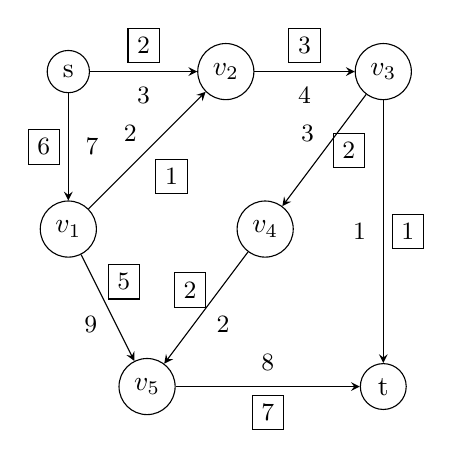
\begin{tikzpicture}[>=stealth, node distance=2cm, every node/.style={draw, circle}]
                % Nodes
                \node[draw] at (0, 0) (s) {s};
                \node[draw] at (0, -2) (v1) {$v_1$};
                \node[draw] at (2, 0) (v2) {$v_2$};
                \node[draw] at (4, 0) (v3) {$v_3$};
                \node[draw] at (2.5, -2) (v4) {$v_4$};
                \node[draw] at (1, -4) (v5) {$v_5$};
                \node[draw] at (4, -4) (t) {t};
        
                % Edges
                \draw[->] (s) -- (v2)
                    node[midway, above, rectangle, yshift = 3pt] {\small 2} 
                    node[midway, below, draw = none] {\small 3};
                    
                \draw[->] (s) -- (v1)
                    node[midway, left, xshift = -3pt, rectangle] {\small 6}
                    node[midway, right, draw = none] {\small 7};
                    
                \draw[->] (v1) -- (v2)
                    node[midway, below right, rectangle, xshift = 3pt, yshift = -3pt] {\small 1}
                    node[midway, above left, draw = none] {\small 2};
                    
                \draw[->] (v1) -- (v5)
                    node[midway, above right, rectangle, yshift = 3pt] {\small 5}
                    node[midway, below left, draw = none] {\small 9};
                
                \draw[->] (v2) -- (v3)
                    node[midway, above, rectangle, yshift = 3pt] {\small 3}
                    node[midway, below, draw = none] {\small 4};
                
                \draw[->] (v3) -- (t)
                    node[midway, right, rectangle, xshift = 3pt] {\small 1}
                    node[midway, left, draw = none] {\small 1};
                
                \draw[->] (v3) -- (v4)
                    node[midway, right, rectangle, xshift = 3pt] {\small 2}
                    node[midway, above left, draw = none] {\small 3};
                
                \draw[->] (v4) -- (v5)
                    node[midway, above left, rectangle] {\small 2}
                    node[midway, below right, draw = none] {\small 2};
                
                \draw[->] (v5) -- (t)
                    node[midway, below, rectangle, yshift = -3pt] {\small 7}
                    node[midway, above, draw = none] {\small 8};
            \end{tikzpicture}
            
            \begin{solution}
                We can see that the best $\Phi_{tot}(F)$ will be $8$ as we can increase the flow along the edge $sv_1$,
                $v_1v_5$ and $v_5t$ to get them to their capacities or closer to,
                e.g.
    
                \begin{figure}[H]
                    \centering
                    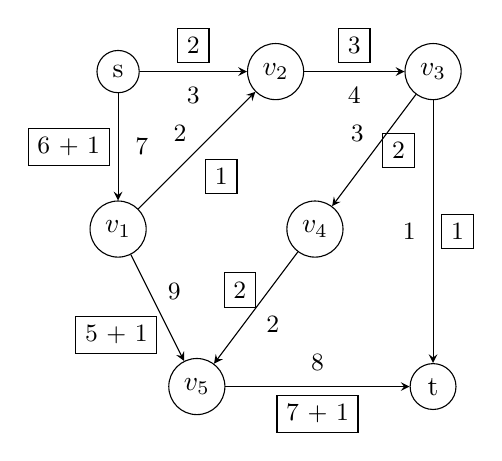
\begin{tikzpicture}[>=stealth, node distance=2cm, every node/.style={draw, circle}]
                        % Nodes
                        \node[draw] at (0, 0) (s) {s};
                        \node[draw] at (0, -2) (v1) {$v_1$};
                        \node[draw] at (2, 0) (v2) {$v_2$};
                        \node[draw] at (4, 0) (v3) {$v_3$};
                        \node[draw] at (2.5, -2) (v4) {$v_4$};
                        \node[draw] at (1, -4) (v5) {$v_5$};
                        \node[draw] at (4, -4) (t) {t};
                
                        % Edges
                        \draw[->] (s) -- (v2)
                            node[midway, above, rectangle, yshift = 3pt] {\small 2} 
                            node[midway, below, draw = none] {\small 3};
                            
                        \draw[->] (s) -- (v1)
                            node[midway, left, xshift = -3pt, rectangle] {\small 6 + 1}
                            node[midway, right, draw = none] {\small 7};
                            
                        \draw[->] (v1) -- (v2)
                            node[midway, below right, rectangle, xshift = 3pt, yshift = -3pt] {\small 1}
                            node[midway, above left, draw = none] {\small 2};
                            
                        \draw[->] (v1) -- (v5)
                            node[midway, below left, rectangle, yshift = -3pt] {\small 5 + 1}
                            node[midway, above right, draw = none] {\small 9};
                        
                        \draw[->] (v2) -- (v3)
                            node[midway, above, rectangle, yshift = 3pt] {\small 3}
                            node[midway, below, draw = none] {\small 4};
                        
                        \draw[->] (v3) -- (t)
                            node[midway, right, rectangle, xshift = 3pt] {\small 1}
                            node[midway, left, draw = none] {\small 1};
                        
                        \draw[->] (v3) -- (v4)
                            node[midway, right, rectangle, xshift = 3pt] {\small 2}
                            node[midway, above left, draw = none] {\small 3};
                        
                        \draw[->] (v4) -- (v5)
                            node[midway, above left, rectangle] {\small 2}
                            node[midway, below right, draw = none] {\small 2};
                        
                        \draw[->] (v5) -- (t)
                            node[midway, below, rectangle, yshift = -3pt] {\small 7 + 1}
                            node[midway, above, draw = none] {\small 8};
                    \end{tikzpicture}
                \end{figure}
        \end{solution}
    \end{figure}
\end{example}

\begin{definition}
    Let $S \subset V$ with $s \in S$ and $t \notin S$.
    Then the cut associated with $S$ is
    \[
    K(S) \coloneqq \{uv \in E\,:\,u \in S, v \in V \setminus S\},
    \]
    i.e.,
    all the directed edges that start in $S$ and finish in $V \setminus S$.
    The capacity of $K(S)$ is
    \[
    \kappa(S) \coloneqq \sum_{e \in K(S)}c_e = \sum_{u \in S, v \in V \setminus S}c_{uv}.
    \]
\end{definition}

The above is saying we cut the graph such that we separate $s$ from $t$.

\begin{example}
    Here is an example of a cut:
    \begin{figure}[H]
        \centering
        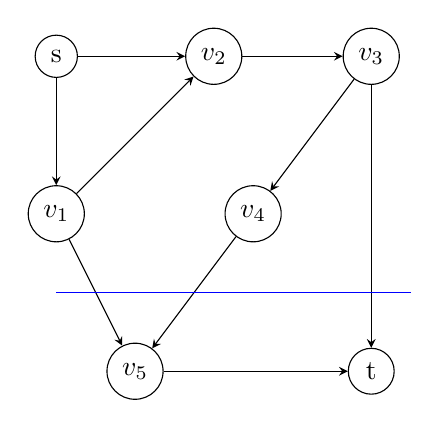
\begin{tikzpicture}[>=stealth, node distance=2cm, every node/.style={draw, circle}]
            % Nodes
            \node[draw] at (0, 0) (s) {s};
            \node[draw] at (0, -2) (v1) {$v_1$};
            \node[draw] at (2, 0) (v2) {$v_2$};
            \node[draw] at (4, 0) (v3) {$v_3$};
            \node[draw] at (2.5, -2) (v4) {$v_4$};
            \node[draw] at (1, -4) (v5) {$v_5$};
            \node[draw] at (4, -4) (t) {t};
    
            % Edges
            \draw[->] (s) -- (v2);
            \draw[->] (s) -- (v1);
            \draw[->] (v1) -- (v2);
            \draw[->] (v1) -- (v5);
            \draw[->] (v2) -- (v3);
            \draw[->] (v3) -- (t);
            \draw[->] (v3) -- (v4);
            \draw[->] (v4) -- (v5);
            \draw[->] (v5) -- (t);

            % Cut
            \draw[blue] (0, -3) -- (4.5, -3);              
        \end{tikzpicture}
    \end{figure}
\end{example}


\begin{theorem}[Max-flow min-cut]
    Given a capacitated network $(V, C)$,
    \[
    \max_{F}\phi_{\text{tot}}(F) = \min_{S}\kappa(S),
    \]
    i.e.,
    the maximum total value over all flows is equal to the minimum cut capacity of the network.
\end{theorem}

\begin{example}
    With these cuts we can see that
    \begin{figure}[H]
        \centering
        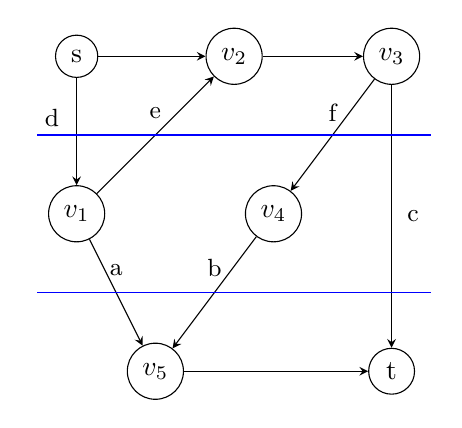
\begin{tikzpicture}[>=stealth, node distance=2cm, every node/.style={draw, circle}]
            % Nodes
            \node[draw] at (0, 0) (s) {s};
            \node[draw] at (0, -2) (v1) {$v_1$};
            \node[draw] at (2, 0) (v2) {$v_2$};
            \node[draw] at (4, 0) (v3) {$v_3$};
            \node[draw] at (2.5, -2) (v4) {$v_4$};
            \node[draw] at (1, -4) (v5) {$v_5$};
            \node[draw] at (4, -4) (t) {t};
    
            % Edges
            \draw[->] (s) -- (v2);
            \draw[->] (s) -- (v1)
                node[midway, left, yshift=5pt, draw=none] {\small d};
            \draw[->] (v1) -- (v2)
                node[midway, above, draw=none] {\small e};
            \draw[->] (v1) -- (v5)
                node[midway, above, draw=none] {\small a};
            \draw[->] (v2) -- (v3);
            \draw[->] (v3) -- (t)
                node[midway, right, draw=none] {\small c};
            \draw[->] (v3) -- (v4)
                node[midway, above, draw=none] {\small f};
            \draw[->] (v4) -- (v5)
                node[midway, above, draw=none] {\small b};
            \draw[->] (v5) -- (t);

            % Cut
            \draw[blue] (-0.5, -3) -- (4.5, -3);
            \draw[blue] (-0.5, -1) -- (4.5, -1);
        \end{tikzpicture}
    \end{figure}
    For the bottom cut we have
    \[
    a + b + c \leq \max{F}
    \]
    and for the top cut we would have
    \[
    d - e + f + c \leq \max{F}.
    \]
    These show how the flow in and out is less than the maximum flow.
\end{example}

\begin{example}
    Construct a maximal flow,
    that is,
    a flow for which $\Phi_{\text{tot}}(F)$ is as big as possible.

    \begin{solution}
        \begin{figure}[H]
            \centering
            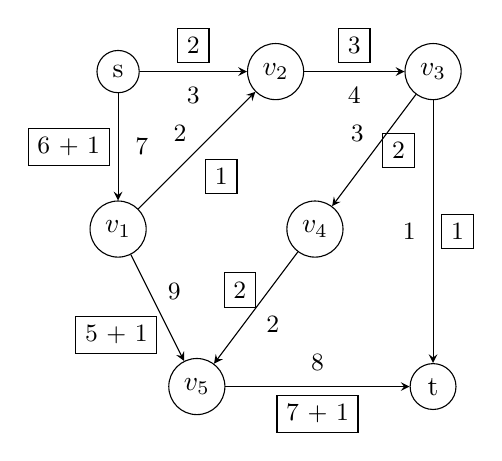
\begin{tikzpicture}[>=stealth, node distance=2cm, every node/.style={draw, circle}]
                % Nodes
                \node[draw] at (0, 0) (s) {s};
                \node[draw] at (0, -2) (v1) {$v_1$};
                \node[draw] at (2, 0) (v2) {$v_2$};
                \node[draw] at (4, 0) (v3) {$v_3$};
                \node[draw] at (2.5, -2) (v4) {$v_4$};
                \node[draw] at (1, -4) (v5) {$v_5$};
                \node[draw] at (4, -4) (t) {t};
        
                % Edges
                \draw[->] (s) -- (v2)
                    node[midway, above, rectangle, yshift = 3pt] {\small 2} 
                    node[midway, below, draw = none] {\small 3};
                    
                \draw[->] (s) -- (v1)
                    node[midway, left, xshift = -3pt, rectangle] {\small 6 + 1}
                    node[midway, right, draw = none] {\small 7};
                    
                \draw[->] (v1) -- (v2)
                    node[midway, below right, rectangle, xshift = 3pt, yshift = -3pt] {\small 1}
                    node[midway, above left, draw = none] {\small 2};
                    
                \draw[->] (v1) -- (v5)
                    node[midway, below left, rectangle, yshift = -3pt] {\small 5 + 1}
                    node[midway, above right, draw = none] {\small 9};
                
                \draw[->] (v2) -- (v3)
                    node[midway, above, rectangle, yshift = 3pt] {\small 3}
                    node[midway, below, draw = none] {\small 4};
                
                \draw[->] (v3) -- (t)
                    node[midway, right, rectangle, xshift = 3pt] {\small 1}
                    node[midway, left, draw = none] {\small 1};
                
                \draw[->] (v3) -- (v4)
                    node[midway, right, rectangle, xshift = 3pt] {\small 2}
                    node[midway, above left, draw = none] {\small 3};
                
                \draw[->] (v4) -- (v5)
                    node[midway, above left, rectangle] {\small 2}
                    node[midway, below right, draw = none] {\small 2};
                
                \draw[->] (v5) -- (t)
                    node[midway, below, rectangle, yshift = -3pt] {\small 7 + 1}
                    node[midway, above, draw = none] {\small 8};
            \end{tikzpicture}
        \end{figure}
        the  minimal cut would be
        \[
        S = \{s, v_1, v_2, v_3, v_4, v_5\}.
        \]
    \end{solution}
\end{example}

For $W \subseteq V$,
define
\[
\phi_{\text{in}}(W) \coloneqq \sum_{u \in V \setminus W}\sum_{v \in W}f_{uv},
\]
the total flow into the set $W$ from vertices outside $W$.
Similarly,
let
\[
\phi_{\text{out}}(W) \coloneqq \sum_{u \in W}\sum_{v \in V \setminus W}f_{uv},
\]
the total flow out of $W$.
With the convention that an empty sum is zero,
note that $\phi_{\text{in}}(V) = \phi_{\text{out}}(V) = 0$
(because there's nowhere outside $V$).

\begin{example}
    Let $W \subset V$ with $y \in V \setminus W$.
    Show that
    \begin{align*}
        \phi_{\text{in}}(W \cup \{y\}) &= \phi_{\text{in}}(W) + \sum_{u \in V \setminus W}f_{uy} - \sum_{v \in W}f_{yv}. \\
        \intertext{Similarly,
        show that}
        \phi_{\text{out}}(W \cup \{y\}) &= \phi_{\text{out}}(W) + \sum_{v \in V \setminus W}f_{yv} - \sum_{u \in W}f_{uy}.
    \end{align*}
    Let $\Delta(W) \coloneqq \phi_{\text{out}}(W) - \phi_{\text{in}}(W)$.

    \begin{solution}
        \begin{align*}
            \phi_{\text{in}}(W \cup \{y\}) &= \phi_{\text{in}}(W) + \phi_{\text{in}}(\{y\}) - \phi_{\text{in}}(W \cap \{y\}) \\
            &= \phi_{\text{in}}(W) + \sum_{u \in V \setminus W}f_{uy} - \text{ flow from $y$ to $W$} \\
            &=\phi_{\text{in}}(W) + \sum_{u \in V \setminus W}f_{uy} - \sum_{v \in W}f_{yv}.
        \end{align*}
        Similarly
        \begin{align*}
            \phi_{\text{out}}(W \cup \{y\}) &= \phi_{\text{out}}(W) + \phi_{\text{out}}(\{y\}) - \phi_{\text{out}}(W \cap \{y\}) \\
            &= \phi_{\text{out}}(W) + \sum_{v \in V \setminus W}f_{yv} - \text{ flow from $W$ to $y$} \\
            &=\phi_{\text{out}}(W) + \sum_{v \in V \setminus W}f_{yv} - \sum_{u \in W}f_{uy}.
        \end{align*}
    \end{solution}
\end{example}

\begin{example}\phantom{}
    \begin{enumerate}[label = (\roman*)]
        \item Show that $\nabla(\{v\}) = 0$ for a single vertex $v \notin \{s, t\}$.

        \item Let $W \subset V$ with $y \in V \setminus W$.
        Use the previous to show that
        \[
        \nabla(W \cup \{y\}) = \nabla(W) + \sum_{v \in V}f_{yv} - \sum_{u \in V}f_{uy}.
        \]

        \item Use induction (i) and (ii) to show that $\nabla(W) = 0$ if $s \notin W$ and $t \notin W$.

        \item Use (ii) and (iii) to show that
        \[
        \nabla(W) = \begin{cases}
            0 & \text{if } s \notin W, t \notin W; \\
            \Phi_{tot}(F) & \text{if } s \in W, t \notin W; \\
            -\Phi_{tot}(F) & \text{if } s \notin W, t \in W; \\
            0 & \text{if } s \in W, t \in W.
        \end{cases}
        \]
    \end{enumerate}

    \begin{solution}\phantom{}
        \begin{enumerate}[label = (\roman*)]
            \item
            From the previous
            \[
            \phi_{in}(W \cup \{y\}) = \phi_{in}(W) + \sum_{u \in V \setminus W}f_{uy} - \sum_{u \in W}f_{yu}
            \]
            \[
            \phi_{out}(W \cup \{y\}) = \phi_{out}(W) + \sum_{u \in V \setminus W}f_{yu} - \sum_{u \in W}f_{uy}.
            \]
            Let $W = \{\}$ any $y = v$.

            \begin{align*}
                \nabla(W \cup \{v\}) &= \phi_{in} - \phi_{out} \\
                &= \phi_{in}(W) + \sum_{u \in V \setminus W}f_{uv} - \left(\sum_{u \in W}f_{vu} + \phi_{out}(W) + \sum_{u \in V \setminus W}f_{vu} - \sum_{u \in W}f_{uv}\right) \\
                \intertext{as $w = \{\}$}
                &= \sum_{u \in V \setminus W}f_{uv} - \sum_{u \in V \setminus W}f_{vu} \\
                &= \sum_{u \in V}f_{uv} - \sum_{u \in V}f_{vu}.
            \end{align*}
            The flow into any vertex is equal to the flow out if it is not $s$ or $t$,
            so
            \[
            \sum_{u \in V}f_{uv} - \sum_{u \in V}f_{vu} = 0
            \]
            such that $v \neq s, t$.

            \item Let $W \subset V$,
            $y \in V \setminus W$.
            \begin{align*}
                \nabla(W \cup \{y\}) &= -\phi_{in} + \phi_{out} \\
                &= -\phi_{in}(W) - \sum_{u \in V \setminus W}f_{uy} + \sum_{u \in W}f_{yu} + \left(\phi_{out}(W) + \sum_{u \in V \setminus W}f_{yu} \cdot \sum_{u \in W}f_{uy}\right) \\
                &= \left(-\phi_{in}(W) + \phi_{out}(W)\right) - \left(\sum_{u \in V \setminus W}f_{uy} + \sum_{u \in W}f_{uy}\right) + \left(\sum_{u \in W}f_{yu} + \sum_{u \in V \setminus W}f_{yu}\right) \\
                &= \nabla(W) - \sum_{u \in V}f_{uy} + \sum_{u \in V}f_{yu}.
            \end{align*}

            \item
            ($1$)
            $w = \{\}, \{v_1\}$,
            $v_1 \neq s, t$.
            ($2$)
            Assume true for $w = \{v_1, \dotsc, v_n\}$,
            $v_i \neq s, t$.
            ($3$)
            $W = \{v_1, \dotsc, v_n\}$ $W = \{v_1, \dotsc, v_n\} \cup \{y\}$ by (ii) $\nabla(W \cup \{y\}) = \nabla W + \sum_{u \in V}f_{yu} - \sum_{u \in V}f_{uy}$,
            by assumption $\nabla W = 0$ and flow into every vertex
            ($\neq s, t$)
            flow out so if $y \neq s, t$ then $\sum_{u \in V}f_{yu} - \sum_{u \in V}f_{uy} = 0$ so $\nabla(W \cup \{y\}) = 0 + 0 = 0$.

            ($4$)
            True for $W = \text{ empty set}$.
            True for $W = \text{ some set $+$ $1$ vertex}$.
            Hence true for all $w$ such that $s, t \notin W$.

            \[
            \nabla(W) = \begin{cases}
                0 & \text{if } s \notin W, t \notin W;\qquad(1) \\
                \Phi_{tot}(F) & \text{if } s \in W, t \notin W;\qquad(2) \\
                -\Phi_{tot}(F) & \text{if } s \notin W, t \in W;\qquad(3) \\
                0 & \text{if } s \in W, t \in W.\qquad(4)
            \end{cases}
            \]
            ($1$) same as (iii)
            ($2$)
            set $y = s$ then $\sum_{u \in V}f_{yu} - \sum_{u \in V}f_{uy} = \Phi_{tot}(F) - 0 = \Phi_{tot}(F)$ as flow out of the source is equal to the total flow,
            so $\nabla(W \cup \{s\}) = \Phi_{tot}(F)$.

            ($4$)
            Take $w_1 = (W \cup \{s\})$,
            $\nabla(W \cup \{s\}) = \Phi_{tot}(F)$,
            take $y = t$
            \[
            \nabla(w_1 \cup \{t\}) = \nabla(w_1) + \sum_{u \in V}f_{tu} - \sum_{u \in V}u_t = \Phi_{tot}(F) + 0 - \Phi_{tot}(F) = 0
            \]
            as flow into sink is equal to the flow out of the source.

            ($3$)
            let $y = t$ then $\nabla(W \cup \{t\}) = o(W) + \sum_{u \in V}f_{tu} - \sum_{u \in V}u_t = 0 + 0 - \Phi_{tot}(F)$ as flow into sink equals total flow so $=\Phi_{tot}(F)$.
        \end{enumerate}
    \end{solution}
\end{example}

\begin{theorem}
    Given a network $(V, C)$,
    \[
    \max_{F}\Phi_{\text{tot}}(F) = \min_{S}\kappa(S),
    \]
    i.e.,
    the maximum total value over all flows is equal to the minimum cut capacity of the network.
\end{theorem}

We have shown that for any $S$-cut,
the total value of a flow satisfies the following
\[
\Phi_{\text{tot}}(F) = \sum_{u \in S, v \in V \setminus S}(f_{uv} - f_{vu}),
\]
and hence $\Phi_{\text{tot}}(F) \leq \min_S\kappa(S)$ for every flow $F$.

\begin{example}
    Here we have constructed a maximal flow:
    
    \textbf{Insert Diagram}.

    
\end{example}

An undirected walk $p$ is a sequence of vertices $s = v_0, v_1, \dotsc$ where for each $r$ at least one of $v_rv_{r + 1}$ or $v_{r + 1}v_r$ is an edge.
One can visit any given vertex as many times as you may wish.

\begin{definition}
    An undirected walk $p = (s = v_0, \dotsc, v_k = t)$ from the source to the sink is called usable if for every successive pair of vertices $v_r, v_{r + 1}$ along the walk,
    at least one of the following holds:
    \begin{enumerate}[label = (\roman*)]
        \item We have $c_{v_r, v_{r + 1}} > 0$ and $c_{v_{r + 1}, v_r} > f_{v_r, v_{r + 1}}$.

        \item We have $c_{v_{r + 1}, v_r} > 0$ and $f_{v_{r + 1}, v_r} > 0$.
    \end{enumerate}
\end{definition}

This is saying,
the walk is usable if for each $r$,
either there is a positive-capacity forwards-oriented edge
(as in $v_r$ to $v_{r + 1}$)
that has spare capacity,
or if there is a positive-capacity backwards-oriented edge
(as in $v_{r + 1}$ to $v_r$)
that has non-zero flow.

It is best to think of the walk as a sequence of vertices,
rather than edges,
to properly understand this definition.

For a vertex $v_r$ in a walk $p$,
let
\[
a(v_r) = \begin{cases}
    c_{v_r, v_{r + 1}} - f_{v_r, v_{r + 1}} & \text{if }c_{v_r, v_{r + 1}} = 0, \\
    c_{v_r, v_{r + 1}} - f_{v_r, v_{r + 1}} + f_{v_{r + 1}, v_r} & \text{if }c_{v_r, v_{r + 1}} > 0.
\end{cases}
\]
So we have $a(v_r)$ being equal to the excess capacity of the forwards oriented edge $v_rv_{r + 1}$,
the flow of the backwards-oriented edge $v_{r + 1}v_r$,
or the sum of both if both directed edges are presented.
Then define the availability of a usable walk $p$ to be
\[
A(p) \coloneqq \min_ra(v_r).
\]
\begin{example}
    Here are some usable walks and paths and their availabilities.
\end{example}

\begin{example}
    Suppose you have a flow $F$.
    Show that if you can find a usable path $p$,
    then you can use it to create a new flow,
    $F'$ say,
    with
    \[
    \Phi_{\text{tot}}(F') = \Phi_{\text{tot}}(F) + A(p).
    \]
    I.e.,
    you can create a new flow and it respects the capacity constraints and satisfies the 'no leaks' condition.

    \begin{solution}
        Have a path $p = \{s, v_1, \dotsc, v_n, t\}$ such that $v_i$ forms a path $i \leq 1 \leq n$,
        then we have
        \[
        A(p) = \min_r{a(v_r)} = \min\{(c_{sv_1} - f_{sv_1}), (c_{v_1v_2} - f_{v_1v_2}), \dotsc (c_{v_nt} - f_{v_nt})\}
        \]
        which implies we have availability in the path so we can create the new flow
        \[
        \Phi_{\text{tot}}(F') = \Phi_{\text{tot}}(F) + A(p).
        \]
    \end{solution}
\end{example}

\begin{example}
    Suppose you have a flow $F$ and there are no usable paths to be found.
    Let $S$ be the set of all vertices that can be reached from $s$ along undirected paths that satisfy the conditions (i) and (ii) in the definition of usable path above.

    Why is $t \notin S$?
    Consider the cut $K(S)$ defined by $S$.
    Prove that $\Phi_{\text{tot}}(F) = \kappa(S)$,
    the capacity of this cut.    
\end{example}

\begin{example}
    Prove the maximum possible total flow is equal to the minimum cut capacity,
    i.e.,
    \[
    \max_{F}\Phi_{\text{tot}}(F) = \min_{S}\kappa(S).
    \]
\end{example}

\begin{example}
    Can we create a maximal flow using the algorithm we gain from identifying a usable path?

    \begin{solution}
        Not always.
        We can only get to $v_1, v_2$ from $s$,
        so there is no usable path between $s$ and $t$.
        Hence this algorithm stops.
        But it is not a maximal flow:

        \begin{figure}[H]
            \centering
            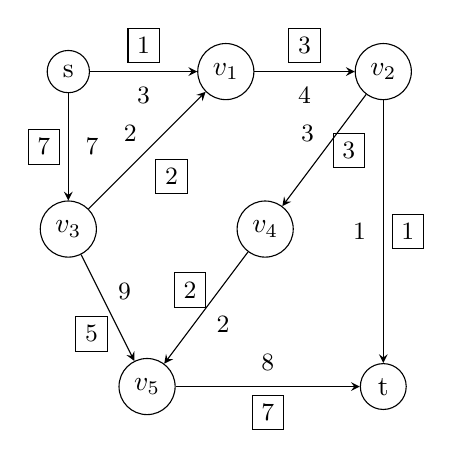
\begin{tikzpicture}[>=stealth, node distance=2cm, every node/.style={draw, circle}]
                % Nodes
                \node[draw] at (0, 0) (s) {s};
                \node[draw] at (0, -2) (v1) {$v_3$};
                \node[draw] at (2, 0) (v2) {$v_1$};
                \node[draw] at (4, 0) (v3) {$v_2$};
                \node[draw] at (2.5, -2) (v4) {$v_4$};
                \node[draw] at (1, -4) (v5) {$v_5$};
                \node[draw] at (4, -4) (t) {t};
        
                % Edges
                \draw[->] (s) -- (v2)
                    node[midway, above, rectangle, yshift = 3pt] {\small 1} 
                    node[midway, below, draw = none] {\small 3};
                    
                \draw[->] (s) -- (v1)
                    node[midway, left, xshift = -3pt, rectangle] {\small 7}
                    node[midway, right, draw = none] {\small 7};
                    
                \draw[->] (v1) -- (v2)
                    node[midway, below right, rectangle, xshift = 3pt, yshift = -3pt] {\small 2}
                    node[midway, above left, draw = none] {\small 2};
                    
                \draw[->] (v1) -- (v5)
                    node[midway, below left, rectangle, yshift = -3pt] {\small 5}
                    node[midway, above right, draw = none] {\small 9};
                
                \draw[->] (v2) -- (v3)
                    node[midway, above, rectangle, yshift = 3pt] {\small 3}
                    node[midway, below, draw = none] {\small 4};
                
                \draw[->] (v3) -- (t)
                    node[midway, right, rectangle, xshift = 3pt] {\small 1}
                    node[midway, left, draw = none] {\small 1};
                
                \draw[->] (v3) -- (v4)
                    node[midway, right, rectangle, xshift = 3pt] {\small 3}
                    node[midway, above left, draw = none] {\small 3};
                
                \draw[->] (v4) -- (v5)
                    node[midway, above left, rectangle] {\small 2}
                    node[midway, below right, draw = none] {\small 2};
                
                \draw[->] (v5) -- (t)
                    node[midway, below, rectangle, yshift = -3pt] {\small 7}
                    node[midway, above, draw = none] {\small 8};
            \end{tikzpicture}
        \end{figure}
        Can only get to $v_1, v_2$ from $s$.
        so no usable path exists between $s$ and $t$.
        Hence this algorithm stops.
        But it is not a maximal flow.
        To increase the flow we can do the following:
        $f_{sv_1} + 1$,
        $f_{st} + 1$,
        $f_{v_3v_1} - 1$,
        $f_{v_3v_5} + 1$ which gives us the maximal flow in the network.
    \end{solution}
\end{example}

Here is another example of us doing the same thing
\begin{example}
    \begin{figure}[H]
        \centering
        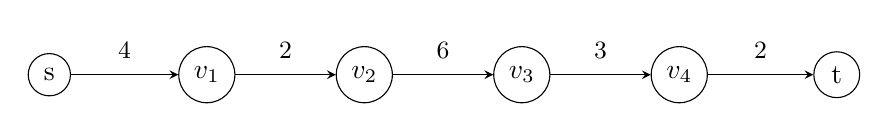
\begin{tikzpicture}[>=stealth, node distance=2cm, every node/.style={draw, circle}]
            % Nodes
            \node[draw] at (-6, 0) (s) {s};
            \node[draw] at (-4, 0) (v1) {$v_1$};
            \node[draw] at (-2, 0) (v2) {$v_2$};
            \node[draw] at (0, 0) (v3) {$v_3$};
            \node[draw] at (2, 0) (v4) {$v_4$};
            \node[draw] at (4, 0) (t) {t};
    
            % Edges
            \draw[->] (s) -- (v1)
                node[midway, above, draw = none] {\small 4};
                
            \draw[->] (v1) -- (v2)
                node[midway, above, draw = none] {\small 2};
                
            \draw[->] (v2) -- (v3)
                node[midway, above, draw = none] {\small 6};
                
            \draw[->] (v3) -- (v4)
                node[midway, above, draw = none] {\small 3};
            
            \draw[->] (v4) -- (t)
                node[midway, above, draw = none] {\small 2};
        \end{tikzpicture}
    \end{figure}
    The path is $\{s, v_1, v_2, v_3, v_4, t\}$,
    then we have the availability of the path:
    \[
    A_p = \{4, 2, 6, 3, 2\}.
    \]
    $\min{A_p} = 2$,
    i.e. the minimum availability is $2$.

    So we can add two to each flow:
    \begin{figure}[H]
        \centering
        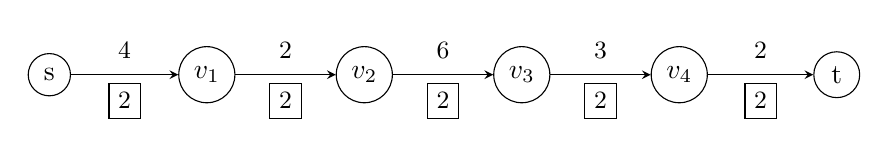
\begin{tikzpicture}[>=stealth, node distance=2cm, every node/.style={draw, circle}]
            % Nodes
            \node[draw] at (-6, 0) (s) {s};
            \node[draw] at (-4, 0) (v1) {$v_1$};
            \node[draw] at (-2, 0) (v2) {$v_2$};
            \node[draw] at (0, 0) (v3) {$v_3$};
            \node[draw] at (2, 0) (v4) {$v_4$};
            \node[draw] at (4, 0) (t) {t};
    
            % Edges
            \draw[->] (s) -- (v1)
                node[midway, above, draw = none] {\small 4}
                node[midway, below, rectangle, yshift = -3pt] {\small 2};
                
            \draw[->] (v1) -- (v2)
                node[midway, above, draw = none] {\small 2}
                node[midway, below, rectangle, yshift = -3pt] {\small 2};
                
            \draw[->] (v2) -- (v3)
                node[midway, above, draw = none] {\small 6}
                node[midway, below, rectangle, yshift = -3pt] {\small 2};
                
            \draw[->] (v3) -- (v4)
                node[midway, above, draw = none] {\small 3}
                node[midway, below, rectangle, yshift = -3pt] {\small 2};
            
            \draw[->] (v4) -- (t)
                node[midway, above, draw = none] {\small 2}
                node[midway, below, rectangle, yshift = -3pt] {\small 2};
        \end{tikzpicture}
    \end{figure}
    so we end with $\min(A_p) = 0$.
\end{example}

\begin{example}
    At the start,
    we assumed that $c_{uu} = 0$,
    i.e.,
    there were no self-loops in he network.
    We also assumed all the capacities were integers.
    Did either of these assumptions matter?

    \begin{solution}
        Assume $c_{uu} = 0$.
        This should not matter as:
        \[
        \Phi_{\text{in}} - \Phi_{\text{out}} = 0
        \]
        for not $s, t$ with $c_{uu} \neq 0$
        \[
        \Phi_{\text{in}} + f_{uu} - \Phi_{\text{out}} - f_{uu} = 0.
        \]

        The fact that the capacities are integers should not matter as we can work as though they are scaled integers,
        e.g. $0.1$ as a capacity would be $1$ if we scaled every capacity by $\times 10$.
    \end{solution}
\end{example}

\begin{example}
    Write down the natural generalisation of the definition of the flow constraints for a multiple-source,
    multiple-sink network.

    \begin{solution}
        Let us have sources $s_1, \dotsc$ and sinks $t_1, \dotsc$.
        We can imagine that we have a vertex connecting all of the sources,
        say $\alpha$,
        and one connecting all of the sinks,
        say $\beta$.
        Once we have these vertices $\alpha, \beta$ we can treat all of the sources and sinks as normal vertices.
        If we chose all of the edges from $\alpha$ to $s_1, \dotsc$ and give them at least the maximum capacity of $s_1, \dotsc$ and the relevant flow then this would mean we can only have one source $\alpha$.

        We can do similar for $\beta$ our sink,
        allowing us to have a single sink with edges connected to $t_1, \dotsc$ with capacities and flows as before.
    \end{solution}
\end{example}


Suppose we wan to maximise the total flow volume,
that is,
the sum of the net flow into all the sinks.
Can we convert this problem into a maximal flow problem of the type we have already studied,
with a single source and single sink?

One idea if you have $n$ sources,
say $s_1, \dotsc, s_n$,
in a network $G$ is to introduce a new network,
we'll call it $G ^ {*}$,
which is the same as $G$ but with a extra vertex,
let's say $\sigma$,
a 'supersource',
and $n$ new edges from $\sigma$ to each $s_i$.
Simply if there is more than one sink,
our new graph $G ^ {*}$ will have a new 'supersink' $\tau$ with an edge to it from each of the original sinks;
if $G$ has both multiple sources and multiple sinks,
we'll do both,
and $G ^ {*}$ will have two new vertices.
Call the resulting network an augmented network.

\subsection{Counting Paths and Menger's Theorem}
From now on we will define a network to mean a graph with two distinguished vertices $s$ and $t$ as before,
but as of yet no capacities assigned to the edges.
It is a directed network if the edges have a direction marked,
and is called undirected if not.

\begin{definition}
    A path in a network will always refer to a sequence of edges going from $s$ to $t$.
    Two paths are said to be edge disjoint if they share no edges in common
    (though they are allowed to share some vertices).
    A directed path in a directed network must at all times be in the direction of the edges it passes along.
\end{definition}

Let $\mathcal{N}_d = \mathcal{N}_d(G)$ denote the number of edge-disjoint directed paths in the directed network $G$.
We will use the max-flow min-cut theorem to prove the following result:

\begin{theorem}\label{sem:disc:thm:mincuteqnumdirected}
    If a directed network $G$ is turned into a capacitated network by declaring that each edge has unit capacity,
    then the number $\mathcal{N}_d$ of edge-disjoint directed paths is equal to the minimal cut capacity,
    i.e.,
    $\mathcal{N}_d = \min_{S}\kappa(S)$.
\end{theorem}

\begin{example}
    In the setting of the previous theorem,
    show that if we have a flow $F$ on the network,
    then we can construct $\Phi_{\text{tot}}(F)$ edge-disjoint directed paths from the source to the sink;
    explain the relevance of the flow constraint to the edge-disjointness.
    Hence show that $\mathcal{N}_d \geq \max_{F}\Phi_{\text{tot}}(F)$.

    \begin{solution}
        As each edge has unit capacity adding a path from $s$ to $t$ set $c_{uv} = f_{uv}$ for $u, v$ in the path.

        Hence $\Phi_{\text{tot}}(F) = \text{Number of paths for a given flow}$ as each path "fills" the capacity of each edge so they must be disjoint.
        So for any flow there is at least $\Phi_{\text{tot}}(F)$ edge disjoint paths.
        I.e.
        \[
        \mathcal{N}_d \geq \max_{F}\Phi_{\text{tot}}(F)
        \]
    \end{solution}
\end{example}

\begin{example}
    Once again,
    in the setting of the previous theorem,
    show that any cut $K(S)$ constrains the maximum number of edge-disjoint paths.
    In particular,
    show that $\mathcal{N}_d \leq \min_{S}\kappa(S)$.

    \begin{solution}
        We have $K(S) \coloneqq \{uv \in E\,:\, u \in S,\, v \in V \setminus S\}$,
        $S \subset V$ so $s \in S$,
        $t \notin S$.
        By the previous example
        \[
        K(S) \geq \mathcal{N}_d \geq \max_F\Phi_{\text{tot}}(F)
        \]
        From max-flow min-cut we get
        \[
        \min_S\kappa(S) = \max_F\Phi_{\text{tot}}(F).
        \]
        Hence
        \[
        \mathcal{N}_d \min_S\kappa(S)
        \]
        

        The paths are edge disjoint and need to go from $s$ to $t$.
        And $s \in S$ so the path needs to go from $S$ to some $v \in V \setminus S$.
        Each path is edge disjoint so once one edge is used from $S$ to $v \in V \setminus S$ it cannot be used again.
        Hence $K(S) \geq \text{Number of edge disjoint paths} = \mathcal{N}_d$.
    \end{solution}
\end{example}

We can turn to the case of undirected networks.
There is a classical theorem for this type of problem
\begin{theorem}[Menger's Theorem]
    The maximum number of edge-disjoint paths from $s$ to $t$ in an undirected graph is equal to the minimal number of edges whose removal leaves no path from $s$ to $t$.
\end{theorem}

\begin{example}
    Consider an undirected network.
    Can you find a way to count the number of edge disjoint paths from $s$ to $t$,
    by relating the problem to an appropriate problem on a directed network?

    \begin{solution}
        \begin{figure}[H]
            \centering
            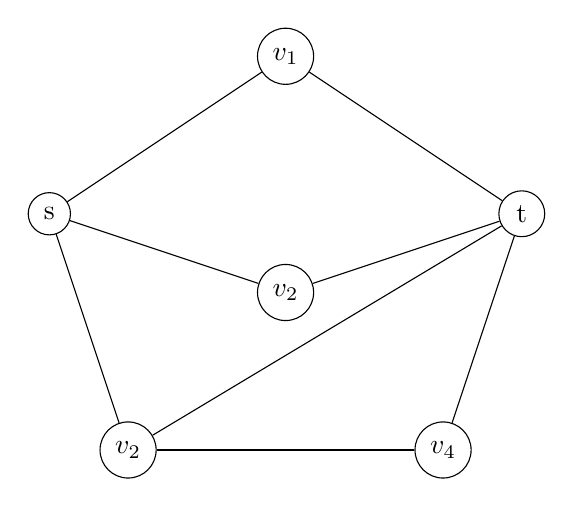
\begin{tikzpicture}[>=stealth, node distance=2cm, every node/.style={draw, circle}]
                % Nodes
                \node[draw] at (-3, 3) (s) {s};
                \node[draw] at (0, 5) (v1) {$v_1$};
                \node[draw] at (0, 2) (v2) {$v_2$};
                \node[draw] at (-2, 0) (v3) {$v_2$};
                \node[draw] at (2, 0) (v4) {$v_4$};
                \node[draw] at (3, 3) (t) {t};
        
                % Edges
                \draw[-] (s) -- (v1);
                
                \draw[-] (s) -- (v2);
                
                \draw[-] (v1) -- (t);
                
                \draw[-] (v2) -- (t);
                
                \draw[-] (s) -- (v3);
                
                \draw[-] (v3) -- (t);
                
                \draw[-] (v3) -- (v4);
                
                \draw[-] (v4) -- (t);
            \end{tikzpicture}
        \end{figure}
        for all $uv$ with $u, v \in V$.
        Add two directed edges one from $uv$ an another from $vu$
        (both ways).
        Using \autoref{sem:disc:thm:mincuteqnumdirected} get the number of edge disjoint paths and figure out the paths.
        \begin{align*}
            p_1 &= \text{path $1$} = \{s, v_1, v_2, \dotsc, u, v, \dotsc, v_n, t\} \\
            p_2 &= \text{path $2$} = \{s, u_1, u_2, \dotsc, v, u, \dotsc, u_n, t\}
        \end{align*}
        with $u, v \in V$ if two paths use $u, v$ swap the paths after that point.
        \begin{align*}
            \tilde{p}_1 &= \{s, v_1, v_2, \dotsc, u, \dotsc, u_n, t\} \\
            \tilde{p}_2 &= \{s, u_1, u_2, \dotsc, v, \dotsc, v_n, t\}.
        \end{align*}
        Repeat until no more $u, v \in V$ such that $uv$ and $vu$ is used.
        E.g.
        \begin{figure}[H]
            \centering
            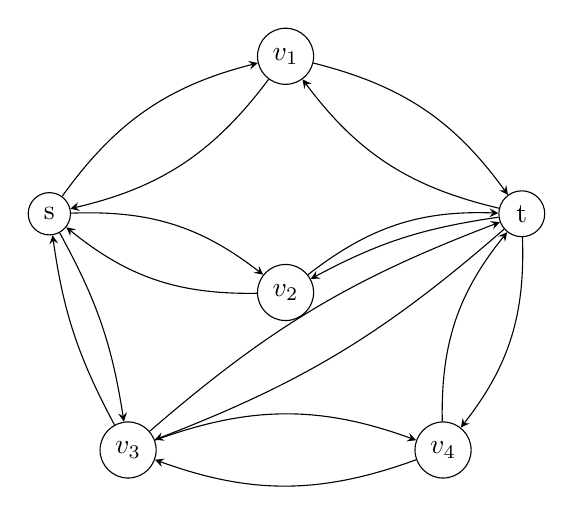
\begin{tikzpicture}[>=stealth, node distance=2cm, every node/.style={draw, circle}]
                % Nodes
                \node[draw] at (-3, 3) (s) {s};
                \node[draw] at (0, 5) (v1) {$v_1$};
                \node[draw] at (0, 2) (v2) {$v_2$};
                \node[draw] at (-2, 0) (v3) {$v_3$};
                \node[draw] at (2, 0) (v4) {$v_4$};
                \node[draw] at (3, 3) (t) {t};
        
                % Edges
                \draw[->, bend left = 20] (s) to (v1);
                \draw[->, bend left = 20] (v1) to (s);
                
                \draw[->, bend left = 20] (s) to (v2);
                \draw[->, bend left = 20] (v2) to (s);
                
                \draw[->, bend left = 20] (v1) to (t);
                \draw[->, bend left = 20] (t) to (v1);
                
                \draw[->, bend left = 20] (v2) to (t);
                \draw[->, bend right = 10] (t) to (v2);
                
                \draw[->, bend left = 10] (s) to (v3);
                \draw[->, bend left = 10] (v3) to (s);
                
                \draw[->, bend left = 10] (v3) to (t);
                \draw[->, bend left = 10] (t) to (v3);
                
                \draw[->, bend left = 20] (v3) to (v4);
                \draw[->, bend left = 20] (v4) to (v3);
                
                \draw[->, bend left = 20] (v4) to (t);
                \draw[->, bend left = 20] (t) to (v4);
            \end{tikzpicture}
        \end{figure}
    \end{solution}
\end{example}

\begin{example}
    What are the maximum number of directed edge-disjoint paths from $s$ to $t$?
    Does the answer stay the same if we remove the directions on the edges and consider only edge-distinct paths from $s$ to $t$ in the resulting undirected graphs?
\end{example}

\begin{theorem}
    The maximum number of edge-disjoint paths from $s$ to $t$ in an undirected graph is equal to the minimal number of edges whose removal leaves no path from $s$ to $t$.
\end{theorem}

\begin{example}
    Consider an undirected network.
    Can you find a way to count the number of edge-disjoint paths from $s$ to $t$,
    by relating the problem to an appropriate problem n a directed network?
\end{example}

\begin{example}
    What are the maximum number of directed edge-disjoint paths from $s$ to $t$?
    Do the answers stay the same if we remove the directions on the edges and consider only edge-distinct paths from $s$ to $t$ in the resulting undirected graphs?
\end{example}

\begin{example}
    Let $K_n$ be the complete graph on $n$ vertices.
    Pick two
    (disjoint)
    vertices and call them $s$ and $t$.
    What is the maximum number of
    (undirected)
    edge-disjoint paths in $K_n$ from $s$ to $t$?

    \begin{solution}
        The number of ways out of $s$ is $n - 1$
        (for $K_n$)
        each can go directly to $t$ since the graph is complete.
    \end{solution}
\end{example}

\begin{example}
    \begin{enumerate}[label = (\roman*)]
        \item Let $K_{n, m}$ be the complete bipartite graph with $n$ 'source' vertices and $m$ 'sink' vertices.
        The edges are directed and all flow from a source vertex to a sink vertex.
        Form an augmented network with one 'supersource' $\sigma$ and one 'supersink' $\tau$.
        Calculate the maximum number of edge-disjoint paths that go from $\sigma$ to $\tau$.

        \item Continuing from (i),
        what is the largest number of edges that can be removed from $K_{n, m}$ and still have the same number of directed edge disjoint paths from $\sigma$ to $\tau$?

        \item What is the maximum number of edges you can allow your enemy to remove from $K_{n, m}$ before he is able to decrease the number of directed edge-disjoint paths from $\sigma$ to $\tau$?
    \end{enumerate}

    \begin{solution}
        \begin{enumerate}[label = (\roman*)]
            \item \phantom{}

            \item
            For this we will denote the number of edges that can be removed from $K_{n, m}$ and still have the same number of directed edge disjoint paths from $\sigma$ to $\tau$ as $\mathcal{E}(n, m)$.
            If $n = m$ then we have $\mathcal{E}(n, m) = n(m - 1)$,
            this is because we are removing the edges between each used node.

            If we have $n > m$ then we get
            \begin{align*}
                \mathcal{E}(n, m) &= m(m - 1) + (n - m)m \\
                &= m(m - 1) + (n - m)m + (n - m)
            \end{align*}
            since:
            $m(m - 1)$ - the number of removed edges between each used node,
            $(n - m)m$ - the removed edges between the unused nodes.
            $(n - m)$ - removing the edges between $\sigma$ and $\tau$.

            For $m > n$ we have the same just where we swap all of the $m$s for $n$s due to the 'symmetry' of bipartite graphs.

            \item I will reduce it if they remove an edge from $\tau$ to $m$ if $m < n$,
            or $\sigma$ to $n$ if $n < m$,
            or the result from (ii) $+1$ if they are taking their time.
        \end{enumerate}
    \end{solution}
\end{example}

\begin{definition}
    A matching in a graph $G$ is a subset $W$ of the edges of $G$ with the property that no vertex of $G$ has more than one edge in $W$ incident to it.
\end{definition}

Consider a bipartite graph on vertices $A \cup B$,
where $A \cap B = \emptyset$,
and every edge has one endpoint in $A$ and the other in $B$.

\begin{definition}[Complete Matching]
    A complete matching is a subset $W$ of edges such that every element of $A$ occurs in one edge,
    and every element of $B$ occurs in at most one edge.
\end{definition}

One can think of a complete matching as follows.
The edges in the bipartite graph indicate preferences for each of the vertices in $A$:
vertex $a \in A$ wants to be matched to one of the vertices in $B$ to which it is joined by an edge.

A complete matching exists if all of these preferences can be simultaneously satisfied.

The definition of complete matching is not symmetric in the $A$ and $B$:
elements of $B$ can be left 'unmatched',
and express no preference in the matter!

\begin{remark}
    Clearly a complete matching can only exist if $|A| \leq |B|$.
\end{remark}

We will now convert our graphs into directed graphs.

\begin{definition}[Out-neighbourhood]
    Suppose $G$ is a directed bipartite graph with vertex subsets $A$ and $B$ and all edges flow from $A$ to $B$.
    For each $U \subseteq A$,
    define $i(U) \subseteq B$ by
    \[
    i(U) = \{b \in B\,:\,\text{there is an edge in $G$ running to $b$ for some $u \in U$}\}.
    \]
    We call $i(U)$ the out-neighbourhood of $U$.
\end{definition}

\begin{example}
    In such a graph,
    prove that if there is a complete matching of $A$,
    then we must have
    \[
    |U| \leq |i(U)|,\text{ for all subsets $U$ of $A$}.
    \]
    Note that the previous includes
    (when $U = A$)
    the observation of our remark that we must have $|A| \leq |B|$,
    since $|i(A)| \leq |B|$.
    The remarkable fact about the condition we gave is that it is not only a necessary condition for a perfect matching to exist,
    but also a sufficient one.

    \begin{solution}
        Say we have a bipartite graph $G$ we can divide the two 'sections' into two sets,
        $A$,
        $B$.

        For $|U| = |A|$ this implies that $|i(U)| = |B|$.
        If $|B| < |A|$,
        for each $b \in B$ we can find a $u \in U \subseteq A$ such that there exists an edge $bu \in G$,
        i.e.
        we can go from any $u \in U$ to many $b \in B$.
        Thus we would naturally have
        \[
        |U| < |i(U)|
        \]
    \end{solution}
\end{example}

\begin{theorem}[Hall's Marriage Theorem]
    If $G$ is a bipartite graph with vertex subsets $A$ and $B$ as above,
    then there is a complete matching of $A$ if and only if the condition in the previous example holds.
\end{theorem}











































\end{document}